\section{Exploring Covariance Functions \cite{gp-ml}}


\subsection{Characteristics of covariance functions \cite{gp-ml}}

\subsubsection{Stationarity and isotropicism}
A stationary covariance function is a function of $X - X'$ only, and is invariant to the exact locations of $X$ and $X'$. An isotropic covariance function is a function only of $|X - X'|$, and is is invariant to the direction of $X - X'$. For example, SE \cite{eq:se} is both stationary and isotropic because it is a function of $|X - X'|$ only.

\subsubsection{Symmetry and positive semidefiniteness}
Given a vector of input points ${X_i | i = 1, ..., n}$, the Gram matrix $K$ is the $n \times n$ matrix whose $(i,j)$-th entry is the inner product between $X_i$ and $X_j$. Since our covariance matrix can be represented as inner products of our vectors of inputs, we can represent it as a Gram matrix. The Gram matrix has two key properties, symmetry and positive semidefiniteness:
\begin{equation*}
    \begin{aligned}
        K_{ij} = K_{ji} \\
        X^T K X \geq 0
    \end{aligned}
\end{equation*}

TODO prove positive semidefiniteness, background needed

\subsubsection{Mean square continuity and differentiability}

To understand how smooth the functions drawn from a Gaussian process are, we need to understand how differentiable and continuous they are. A more differentiable function implies that the function contains higher order polynomials which makes it smoother, and a continuous function avoids any reductions in smoothness produced by discontinuities.

Because the functions drawn from the Gaussian distribution are random functions between datapoints, there are infinitely many possible functions and determining if they are all continuous or differentiable is impossible. We are l
Instead, we can examine if the covariance function responsible for producing these functions is differentiable and continuous

\paragraph{Continuity}
Let $x$ be an infinite-length vector of inputs $x_1, x_2, ...$ whose values linearly approach some stable fixed point $x_*$ as the sequence progresses. Formally:
\begin{equation*}
    \lim_{k \to \infty} |x_k - x_*| = 0
\end{equation*}

A regular function $f$ is continuous at $x_*$ if three conditions are met. $x_*$ must exist in the domain of $f$, e.g. $f(X) = 1/x$ is not continuous at $f(0)$ because $0$ is not in the domain of $f$. There must be a single limit the function approaches.
\begin{equation*}
    f(X) = \begin{cases}
        0 & \text{if } X < 0 \\
        1 & \text{if } X > 0 \\
        2 & \text{if } X = 0
    \end{cases}
\end{equation*}
In this example, at $f(0)$ $x$ is not continuous at $x = 0$ since $f$ approaches both $0$ and $1$. This single limit needs to be the same as the function evaluation at the limit. If we removed the $0 \text{ if } X < 0$ case to produce a single limit, it would still not be continuous at $x = 0$ since the limit would be $1$ but $f(0) = 2$. Formally summarising these three ideas:
\begin{equation*}
    \lim_{x \to x_*} |f(x) - f(x_*)| = 0
\end{equation*}

A Gaussian process $f$ is MS continuous at $x_*$ if the expected function evaluations $E[f(x)]$ quadratically approach $f(x_*)$ as $x \to x_*$. Formally:
\begin{equation*}
    \lim_{x \to x_*} \mathbb{E}[(f(x) - f(x_*))^2] = 0
\end{equation*}

The quadratic term in our limit means our mean squared errors will also vary continuously, so we avoid wild "swings" in uncertainty when moving away from training data points in the input space. More importantly, it allows the error term to be expanded directly into kernel terms: 
\begin{equation*}
    \begin{aligned}
        \mathbb{E}[(f(x) - f(x_*))^2] &= \mathbb{E}[f(x)^2] + \mathbb{E}[f(x_*)^2] - 2\mathbb{E}[f(x)f(x_*)] \\
        &= k(x, x) + k(x_*, x_*) - 2k(x, x_*)
    \end{aligned}
\end{equation*}
Using this expansion in our definition of MS continuity: 
\begin{equation*}
    \lim_{x \to x_*} | k(x, x) - 2k(x, x_*) + k(x_*, x_*) | = 0
\end{equation*}
Because $x_*$ is given, $k(x_*, x_*)$ is a constant. This limit requires that both $k(x, x)$ and $k(x, x_*) \to k(x_*, x_*)$ as $x \to x_*$, which is the very definition of continuity of $k$ at $x_*$ - they guarantee that $x_*$ is in the domain of $k$, that it has a single limit, and this limit of $k(x, x_*)$ is $k(x_*, x_*)$ as $x \to x_*$. Therefore, a Gaussian process is MS continuous at $x_*$ if and only if the covariance function $k$ is continuous at $x_*$. For stationary covariance functions, this reduces to checking that $k$ is continuous at $x_* = 0$.

\paragraph{Differentiability}
The MS derivative of $f(X)$ in the $i$th direction is:
\begin{equation*}
    \frac{\delta f(x)}{\delta x_i} = \text{l.i.m}_{h \to 0} \frac{f(x + h e_i) - f(x)}{h}
\end{equation*}

\subsection{Stationary covariance functions \cite{gp-ml}}

\subsubsection{Spectral density for stationary processes}
TODO, background needed

\subsubsection{Squared exponential (SE)}
Here is the already introduced SE:
\begin{equation*}
    k(X,X*) = \exp \left(- \frac{|X - X'|^2}{2l^2} \right)
\end{equation*}

We can find the value for $l$ analytically using \ref{eq:general_l}:
\begin{equation*}
    l = \frac{1}{2\pi\hat{N}_u} \exp\left(-\frac{u^2}{2\sigma^2}\right)
\end{equation*}
Setting $u = 0$ makes our term inside the exponential equal to zero:
\begin{equation*}
    l = \frac{1}{2\pi\hat{N}_0}
\end{equation*}

This covariance function is infinitely differentiable thanks to the $\exp$ term, so a GP using SE is infinitely mean-squared differentiable, which produces very smooth functions.

\begin{figure}[h]
    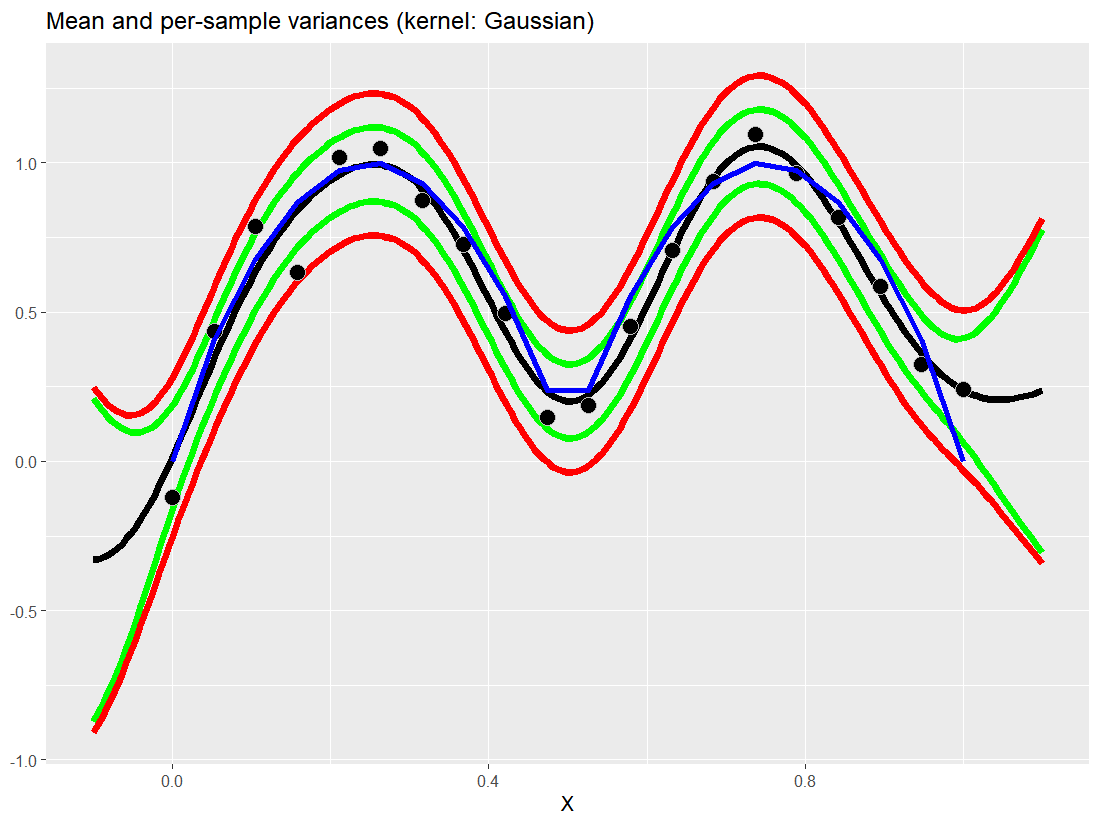
\includegraphics[height=0.5\textwidth]{gaussian_variances.png}
    \caption{
        Plot of a Gaussian process using SE applied to a toy dataset. The toy dataset ($n = 15$) is a data-generating function in blue with some Gaussian noise applied to produce the datapoints in black. The black line represents the expected function from the Gaussian process. The green line represents the 90\% confidence interval around the predictive distribution without the $\sigma^2_n$ term, representing the uncertainty surrounding predictions of the noise-free mean function $f(X)$. The red line represents the 90\% confidence interval with $\sigma^2_n$, representing the uncertainty surrounding predictions of the noisy observations $y$.
    }
\end{figure}

\begin{figure}[h]
    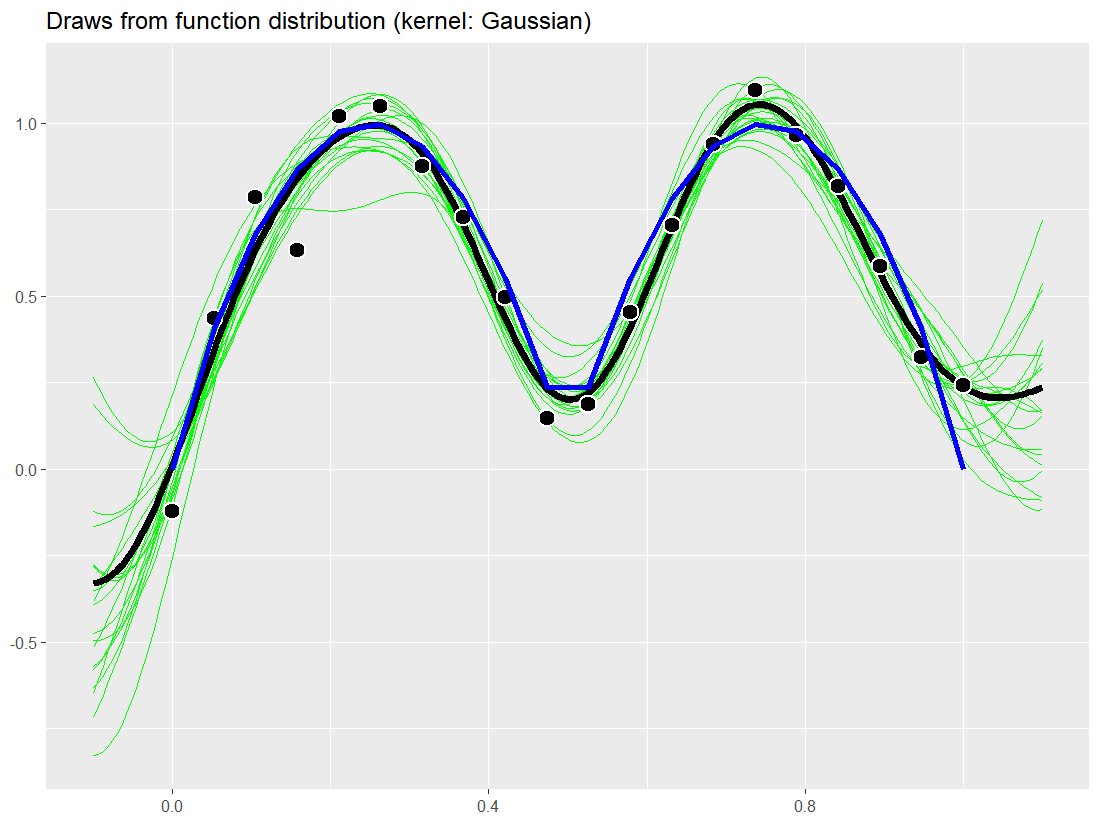
\includegraphics[height=0.5\textwidth]{gaussian_draws.png}
    \caption{
        Plots of functions from a Gaussian process using SE applied to the same toy dataset. The blue line and black datapoints and lines are as before, but the green lines here are a sample of functions drawn from the Gaussian process.
    }
\end{figure}

TODO proof of infinite basis functions


% Often causes issues since it assumes infinite differentiability. Experts don’t recommend using it. \cite{gaopro}

% TODO fix formatting here
\newpage
\subsubsection{Matern-class}
The Matern class of covariance functions is given by:
\begin{equation*}
    k(X,X') = \frac{2^{1 - \nu}}{\Gamma(\nu)}\left(\frac{\sqrt{2\nu}|X - X'|}{l}\right)^{\nu}K_{\nu}\left(\frac{\sqrt{2\nu}|X - X'|}{l}\right)
\end{equation*}

$l$ is our familiar length scale hyperparameter, but $\nu$ controls how differentiable the function is. 

TODO Bessel function $K_{\nu}$, background needed
Therefore, a a Gaussian process using a Matern class kernel is $k$-times MS differentiable if and only if $\nu > k$. 

We can simplify this by using half-integers, i.e. $\nu = p + 1/2$ where $p$ is a non-negative integer. In this case, the covariance function becomes a product of a polynomial and an exponential:

\begin{equation*}
    k_{\nu = p + 1/2}(X,X') = \exp \left(- \frac{\sqrt{2\nu}|X - X'|}{l} \right) \frac{\Gamma(p+1)}{\Gamma(2p+1)} \sum_{i=0}^p \frac{(p + i)!}{i!(p-i)!} \left( \frac{\sqrt{8\nu r}}{l} \right)^{p-i}
\end{equation*}

$\nu = 1/2$ is equivelant to the exponential covariance function.

TODO formula

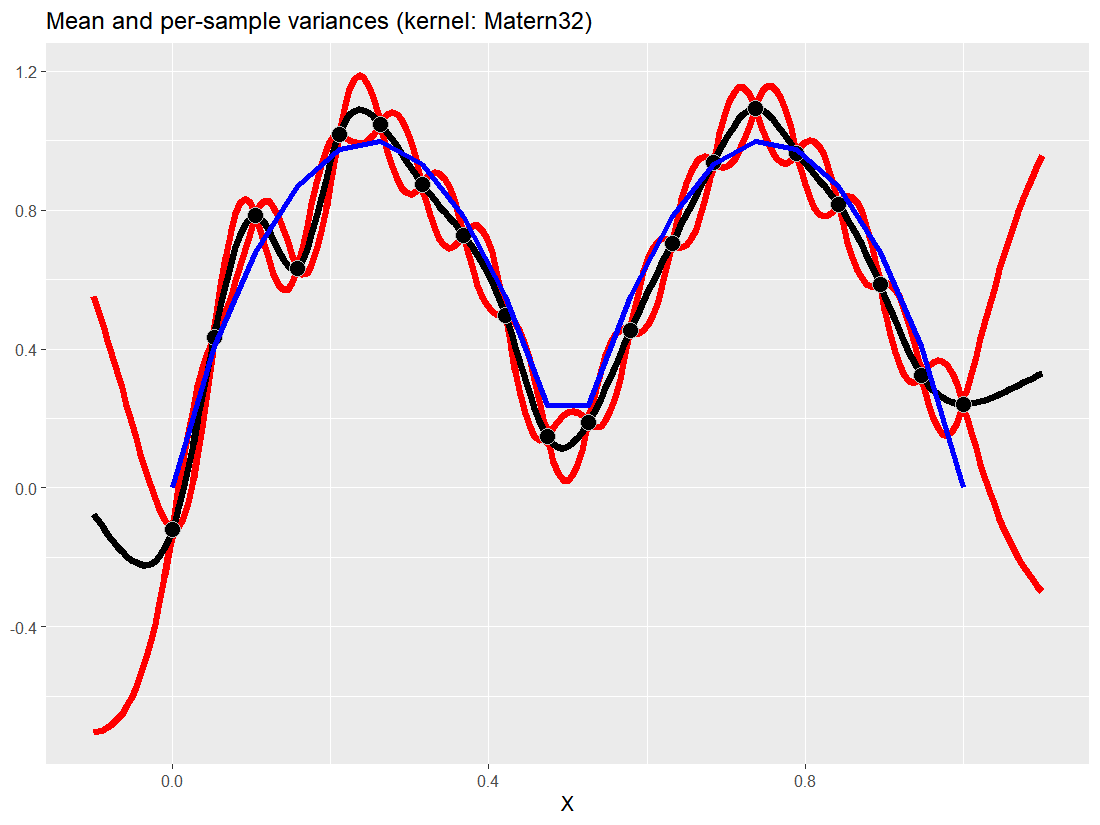
\includegraphics[height=0.5\textwidth]{matern32_variances.png} \\
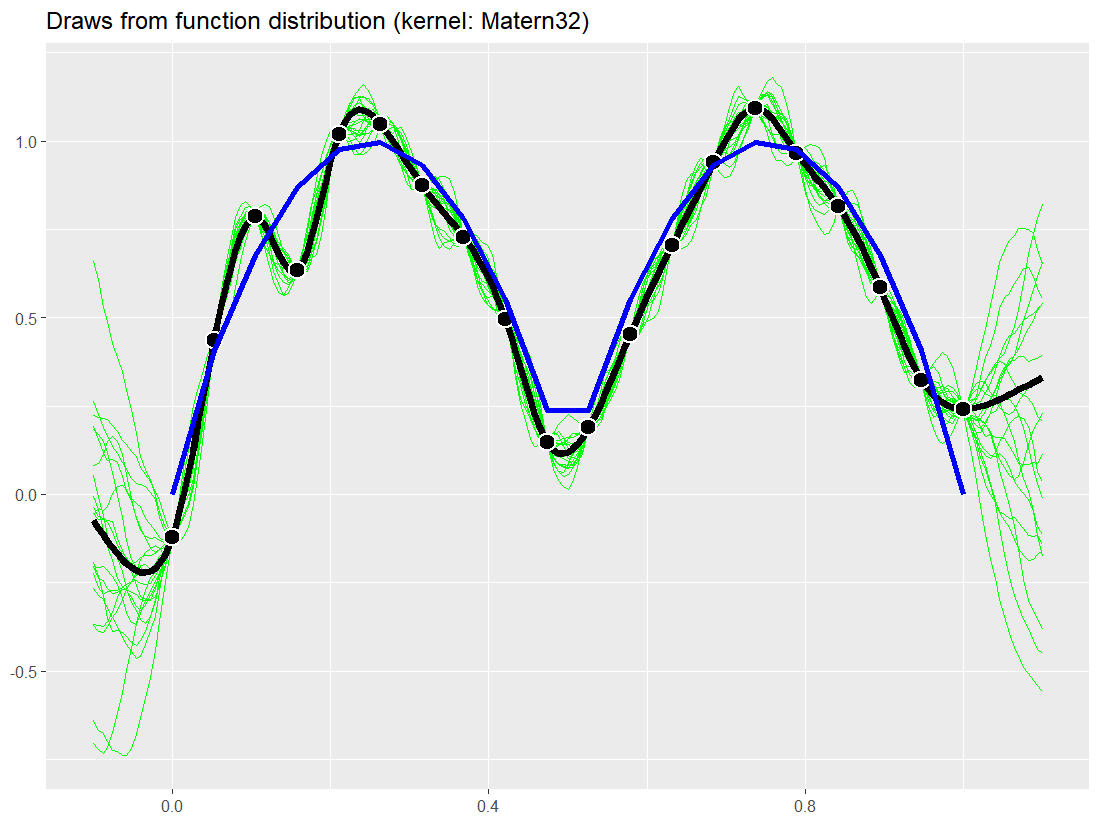
\includegraphics[height=0.5\textwidth]{matern32_draws.png} \\

% Matern 3/2: Assumes one time differentiability. This is often too low of an assumption. \cite{gaopro}

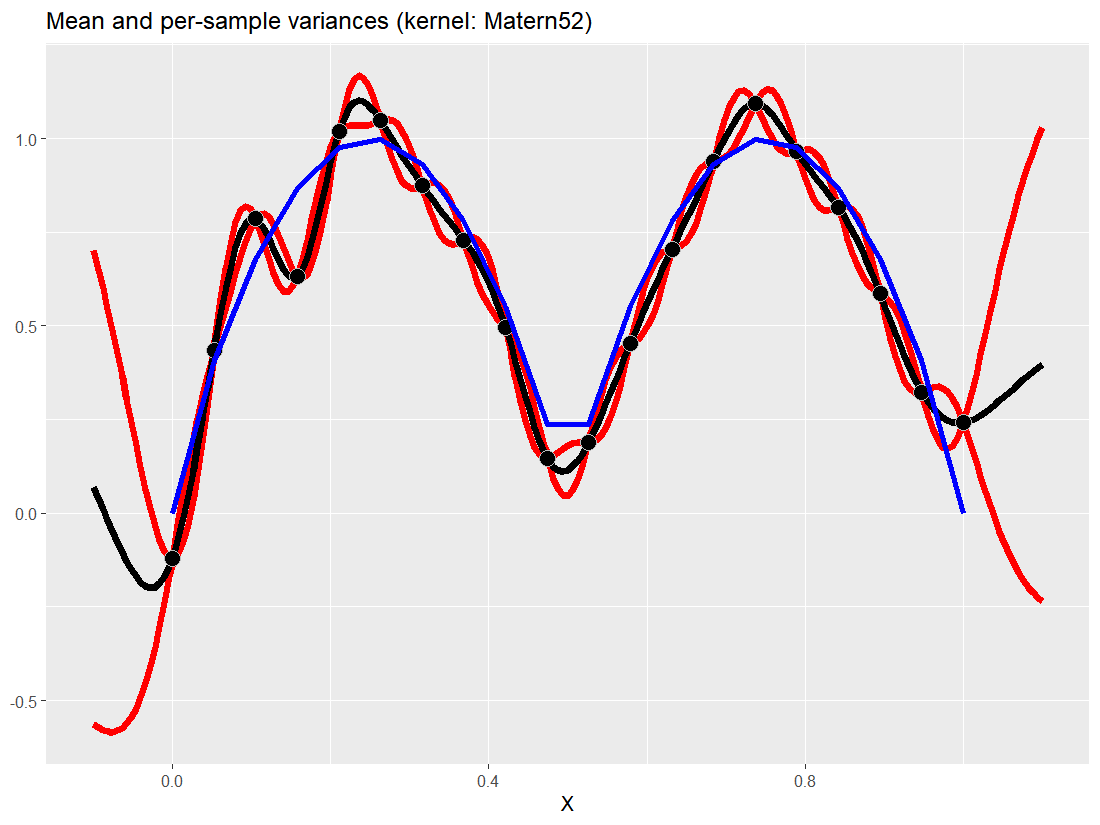
\includegraphics[height=0.5\textwidth]{matern52_variances.png} \\
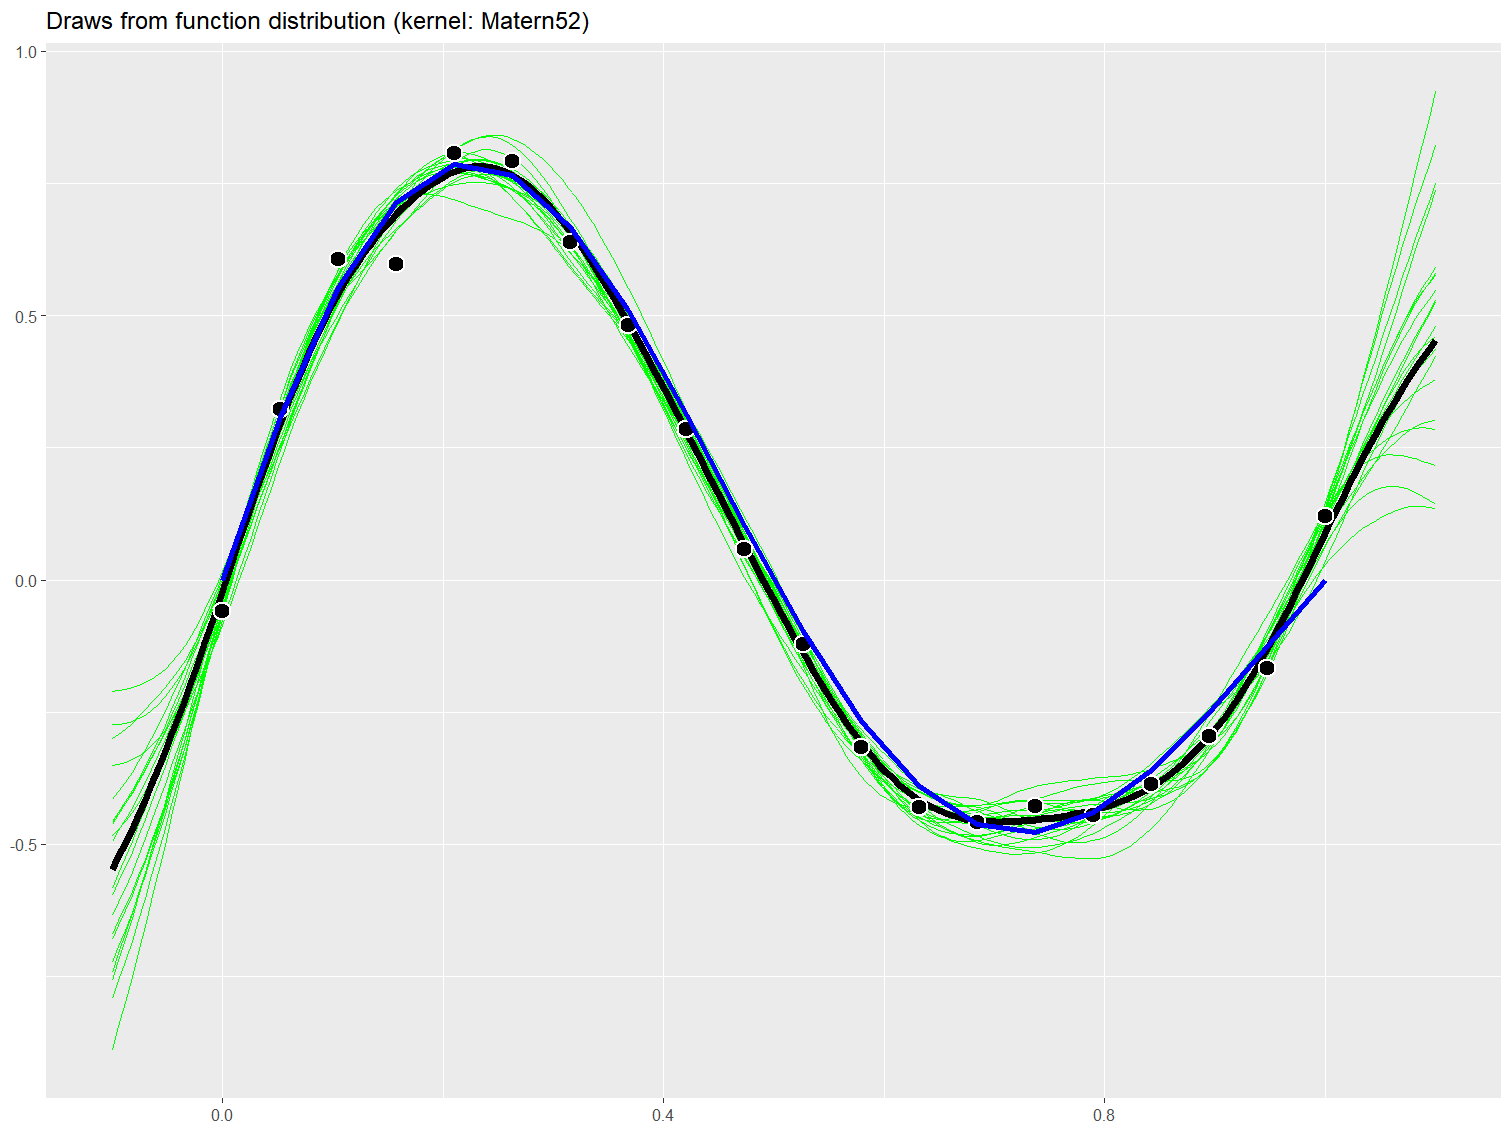
\includegraphics[height=0.5\textwidth]{matern52_draws.png} \\

% Matern 5/2: Assumes two time differentiability. Generally the best. \cite{gaopro}

\subsubsection{Exponential and $\gamma$-exponential}
TODO formulas 

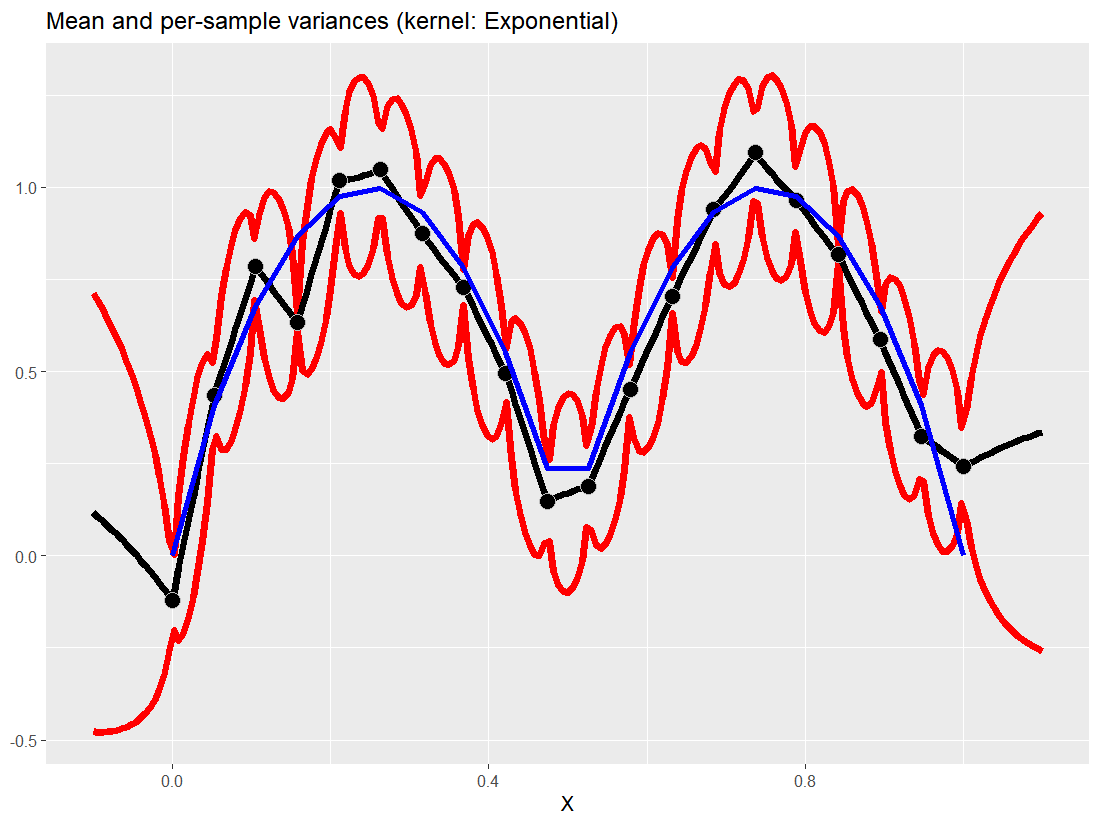
\includegraphics[height=0.5\textwidth]{exp_variances.png} \\
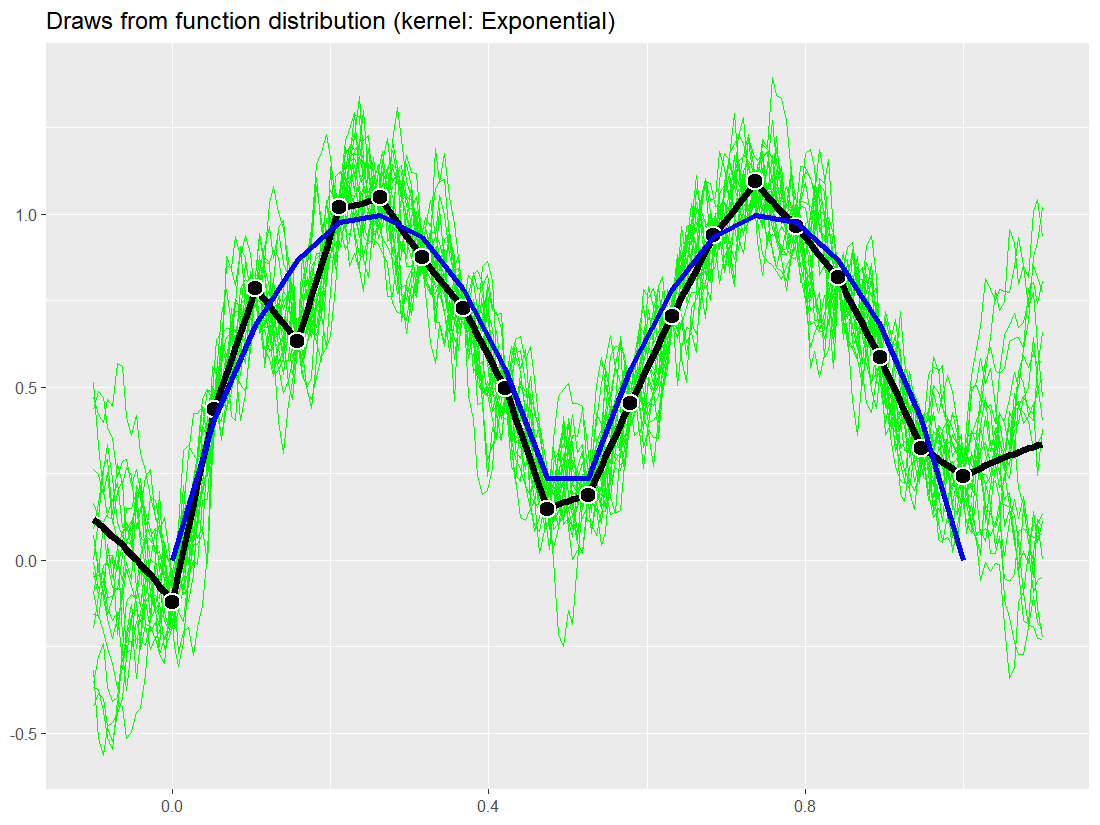
\includegraphics[height=0.5\textwidth]{exp_draws.png} \\
% Exponential: Equivalent to Matern 1/2. Assumes no differentiability. \cite{gaopro}

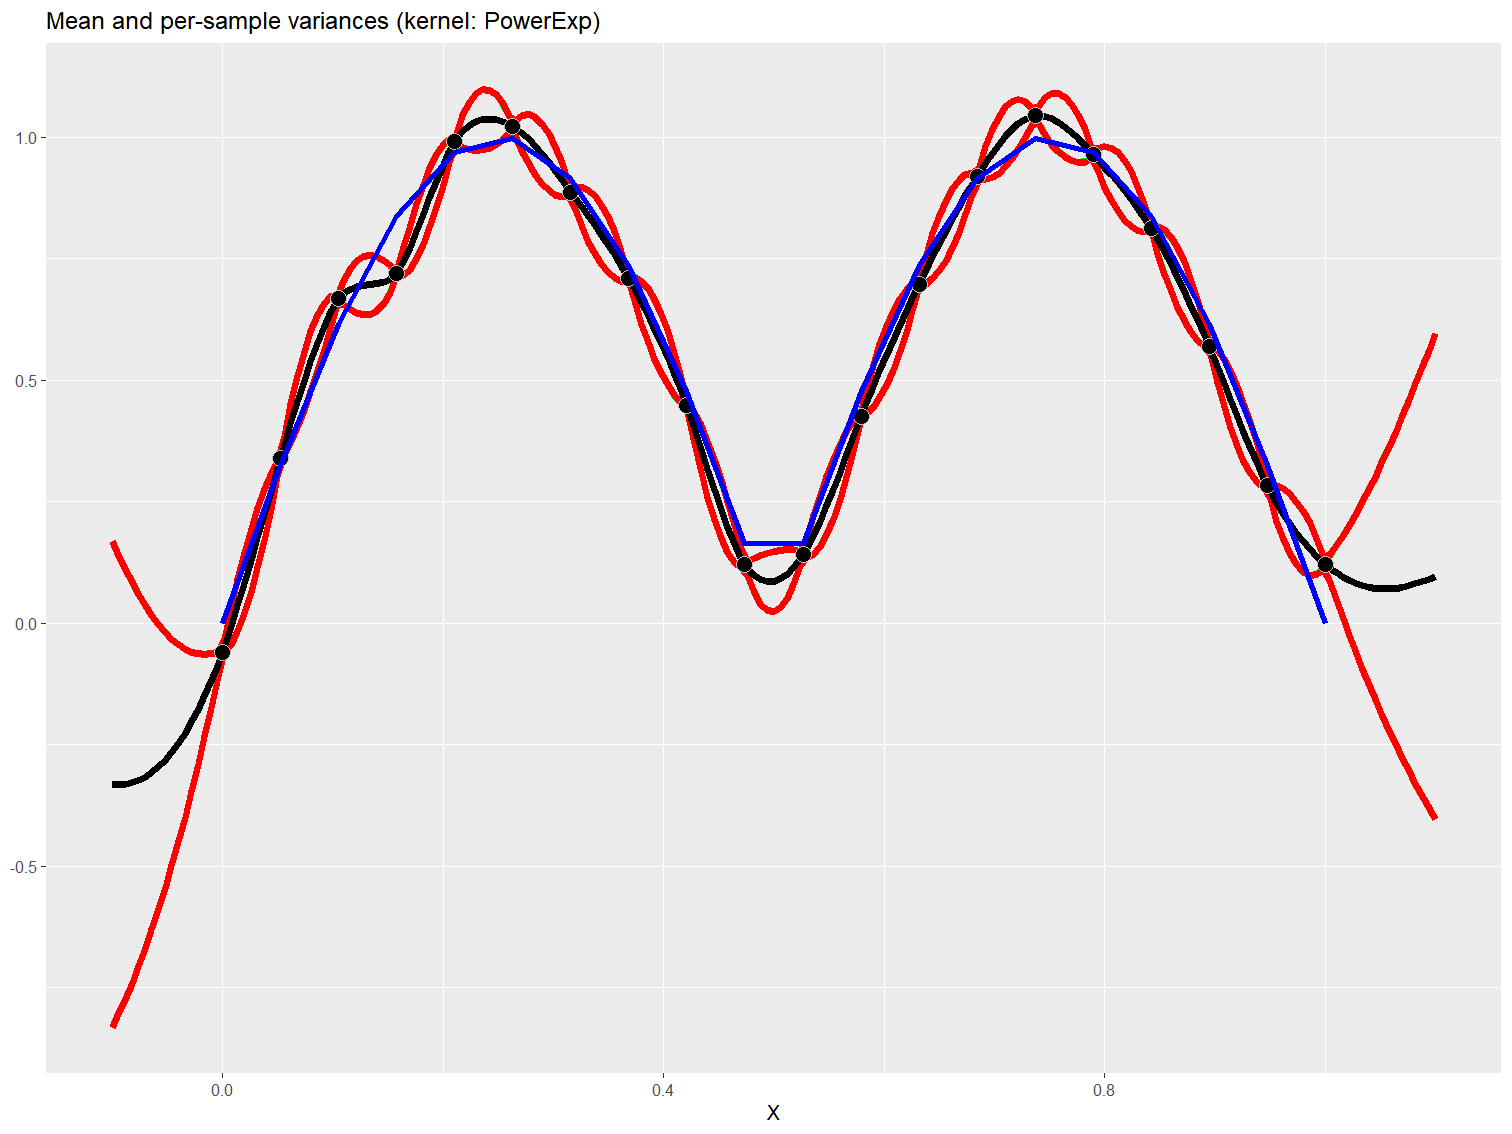
\includegraphics[height=0.5\textwidth]{powerexp_variances.png} \\
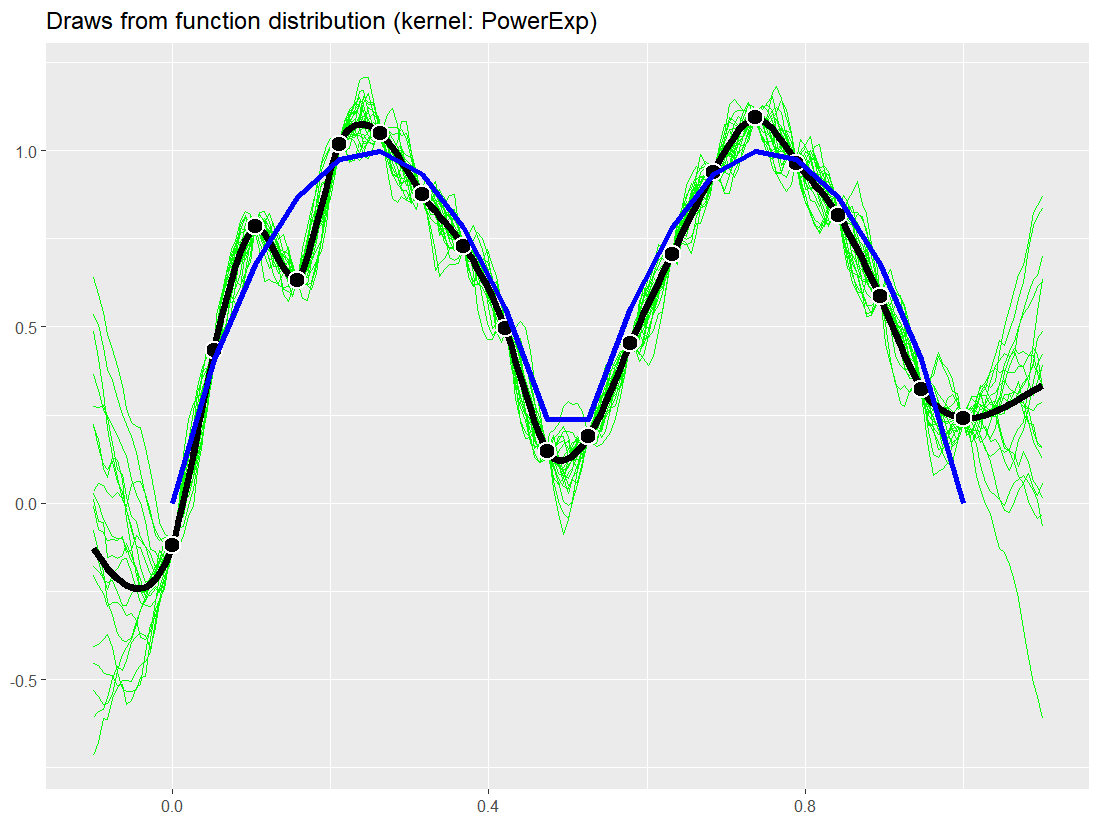
\includegraphics[height=0.5\textwidth]{powerexp_draws.png} \\

\subsubsection{Rational quadratic}
The rational quadratic can be seen as an infinite sum of SE with different length-scales.

TODO formulas

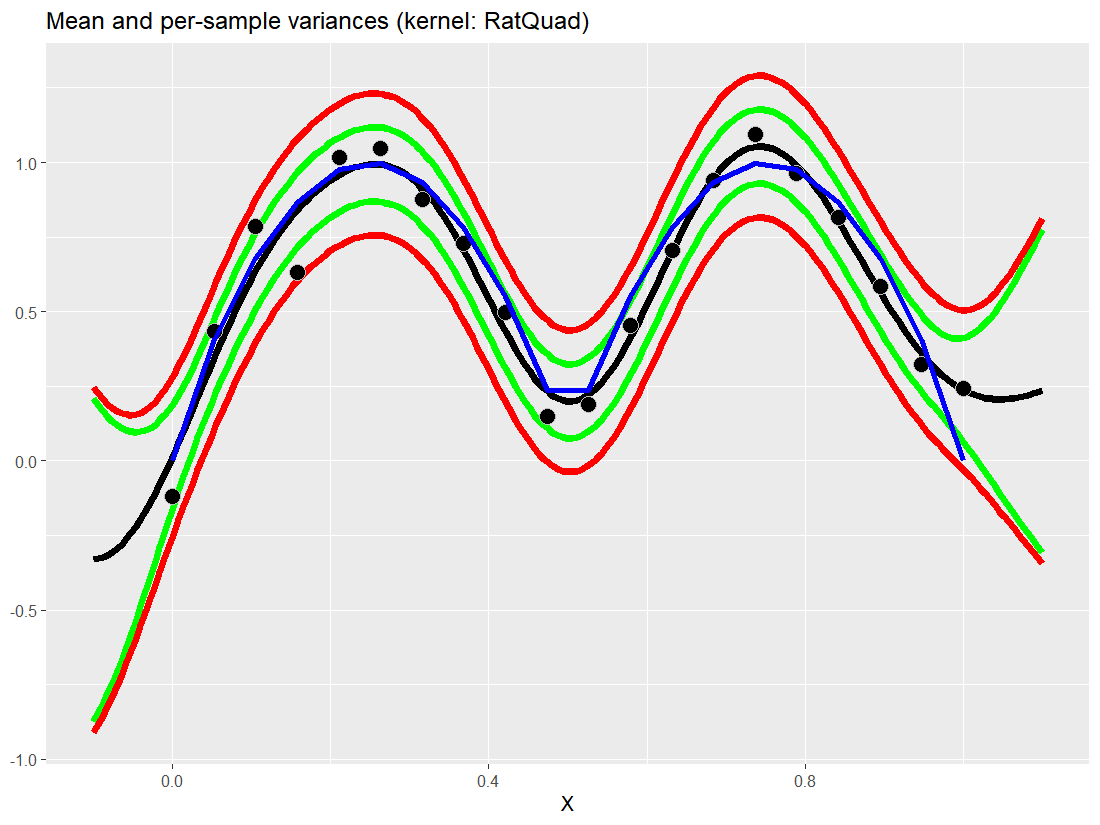
\includegraphics[height=0.5\textwidth]{ratquad_variances.png} \\
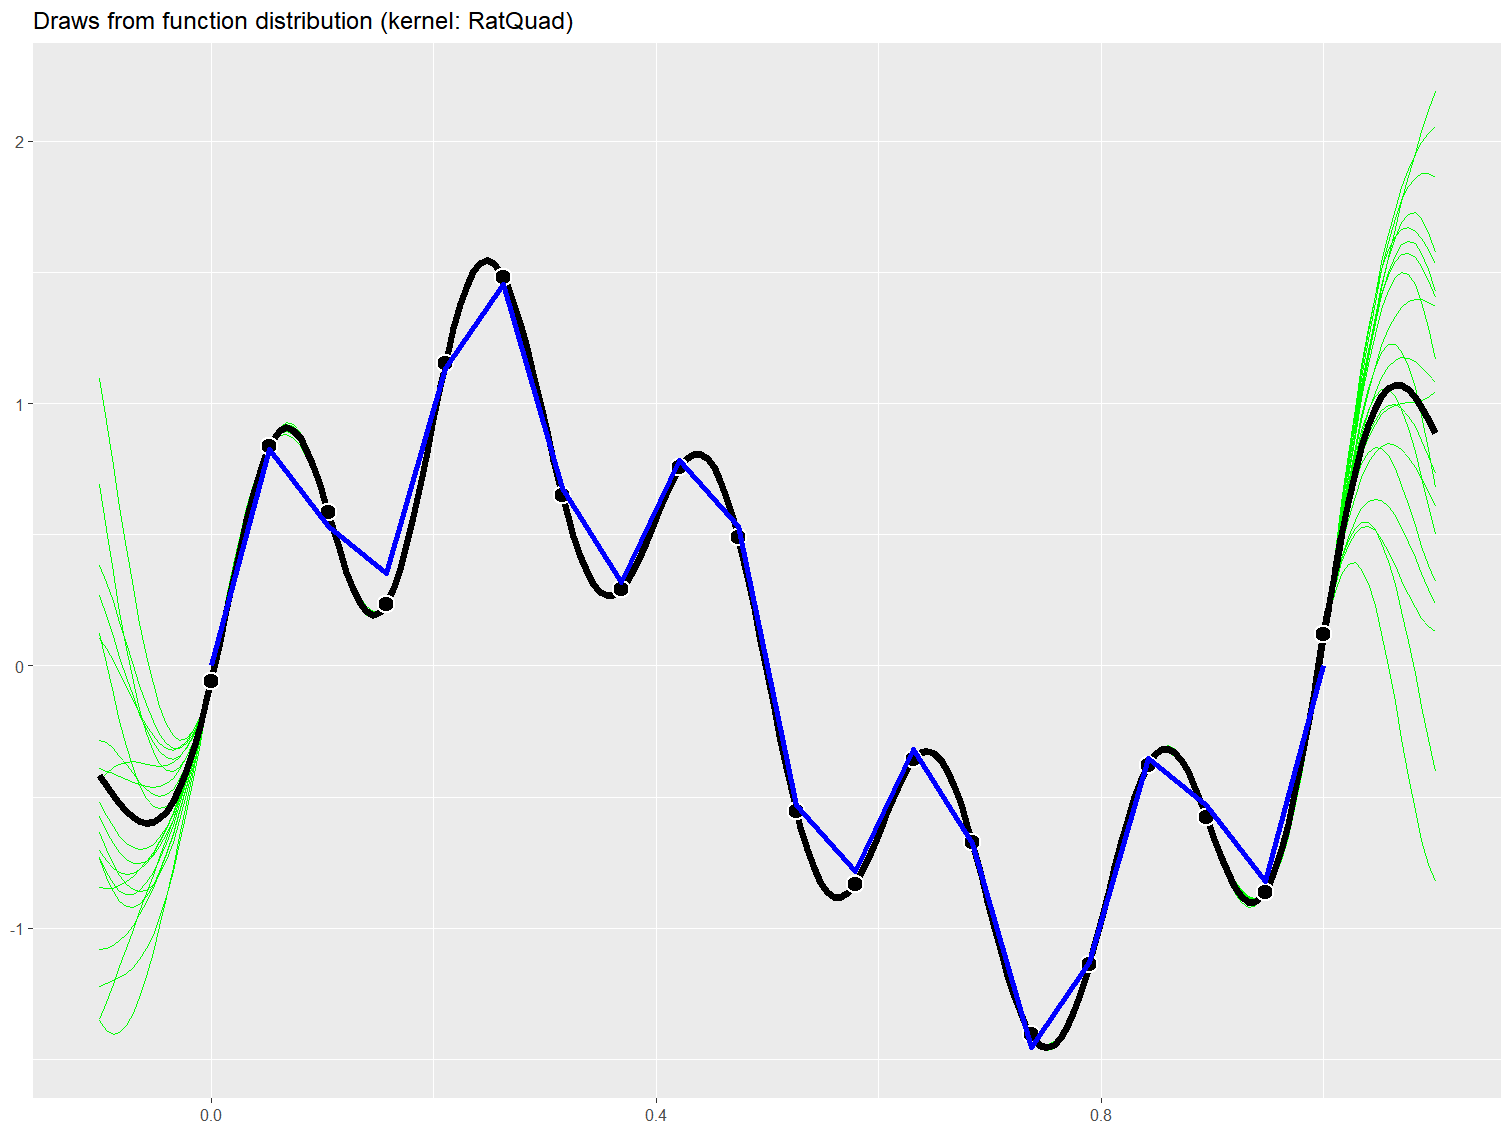
\includegraphics[height=0.5\textwidth]{ratquad_draws.png} \\


% \subsection{Non-stationary covariance functions \cite{gp-ml}}
% 
% \subsubsection{Sum and product}
% 
% \subsubsection{Neural network}
% 
% \subsubsection{Warping and periodicity}


% \subsection{Language-processing covariance functions \cite{gp-ml}}
% 
% \subsubsection{String}
% 
% \subsubsection{Fisher}
% 
% 
% \subsection{Factor-processing covariance functions \cite{gaopro}}
% 
% \subsubsection{Ordered factor}
% 
% \subsubsection{Factor}
% 
% \subsubsection{Gower factor}
% 
% \subsubsection{Indices-ignoring}


\subsection{Deriving kernels \cite{deriving-kernels}}
TODO

\subsection{Learning best kernel from data \cite{choosing-kernels}}
TODO

% \subsection{Additive covariance kernels for high-dimensional learning \cite{additive-kernels}}
% 
% 
% \subsection{Hierarchical Bayesian covariance function for hierarchical modelling \cite{hierarchical-kernels}}
% 
% 
% \subsection{Free-form covariance matrix for multi-task learning \cite{freeform-kernels}}
% 
% 
% \subsection{Combining different kernels for multi-task learning \cite{multi-kernels}}



% \section{Extensions of the Gaussian Process}
% 
% 
% \subsection{Gaussian process regression networks \cite{gprn}}
% 
% 
% \subsection{Variational Gaussian process \cite{vgp}}
